\chapter{Discussion}\label{ch:discussion}

\begin{chapterabstract}
    This chapter begins with the outline of the work done as part of this thesis.
    The following section (\ref{sec:proof-of-concept-implementation}) discusses the proof-of-concept implementation and technical challenges during development and answers research question no.~2.
    Section~\ref{sec:experiments_discussion} then discusses the individual results of experiments conducted in Chapter~\ref{ch:results} and leads to answering research question no.~1.
\end{chapterabstract}

\section{Outline}\label{sec:discussion_outline}

This thesis examined the ideas of federated ecosystems, data spaces, and related concepts.
Special emphasis was placed on the concrete implementation of these ideas --- Gaia-X~\cite{gaiax}.
This work aimed to implement a Gaia-X-compliant data exchange module into the Carecentive~\cite{carecentive} platform based on available Gaia-X specifications and leverage reference implementations and the running GXDCH services.

The implementation process of the data exchange module, acting as a proof of concept, itself served as a way to answer research question 2 --- ``\textit{What are the technical challenges in implementing Gaia-X-compliant software?}'' and is discussed in Section~\ref{sec:proof-of-concept-implementation}.
The functionality of the implementation, Gaia-X services, and the specifications were explored by executing predefined experiments focused on different aspects of the data exchange process.
Those are discussed in Section~\ref{sec:experiments_discussion} and are used to answer research question 1 --- ``\textit{Is it feasible to share healthcare data in Gaia-X Data Spaces?}''.

\section{Proof of concept implementation}\label{sec:proof-of-concept-implementation}

The task of the practical side of the thesis was to implement a Gaia-X-compliant data exchange module into the Carecentive platform.
The reasoning behind this was twofold: (1) to enable the exchange of the palliative care trial data with other parties in a trustworthy and interoperable environment and (2) to assess the current state of the Gaia-X ecosystem and note any technical challenges in the process.

Therefore, a solution was developed and embedded into the Carecentive app to enable the registration of existing data assets into the Gaia-X ecosystem.
From a high-level view, the module was supposed to serve two main functionalities.
Firstly, the Gaia-X Credentials corresponding to objects in Carecentive, which mainly include the Participant credential (corresponding to the Carecentive admin) and the credentials describing the offered data, are created.
Secondly, the goal was to enable some kind of process (contracting, handshake, etc.), serving as a basis for the subsequent data exchange.

However, during the development phase, it became evident that the implementation process was not without its hurdles.
These challenges were primarily linked to the state of the specifications, reference implementation (XFSC), and the GXDCH services.
The specific issues are detailed in the subsequent sections of this report.

\subsection{Specifications}\label{subsec:specifications}

When people first familiarize themselves with Gaia-X's technical and functional specifics, they must decide which specification to review.
This is because the specifications are divided into five different documents; ``Policy Rules Conformity Document,''~\cite{gaiax_policy_rules} ``Architecture Document,''~\cite{gaiax_architecture_document} ``Trust Framework,''~\cite{gaiax_trust_framework} ``Identity and Access Management,''~\cite{gaiax_identity_and_access_management} and ``Data Exchange Document.''~\cite{gaiax_data_exchange_document}
The overview of available specifications is available in Figure~\ref{fig:specifications}.
Initially, it can be very confusing and unclear which document deals with the person's use case, leading to the need to study multiple vast documents.

\begin{figure}
    \centering
    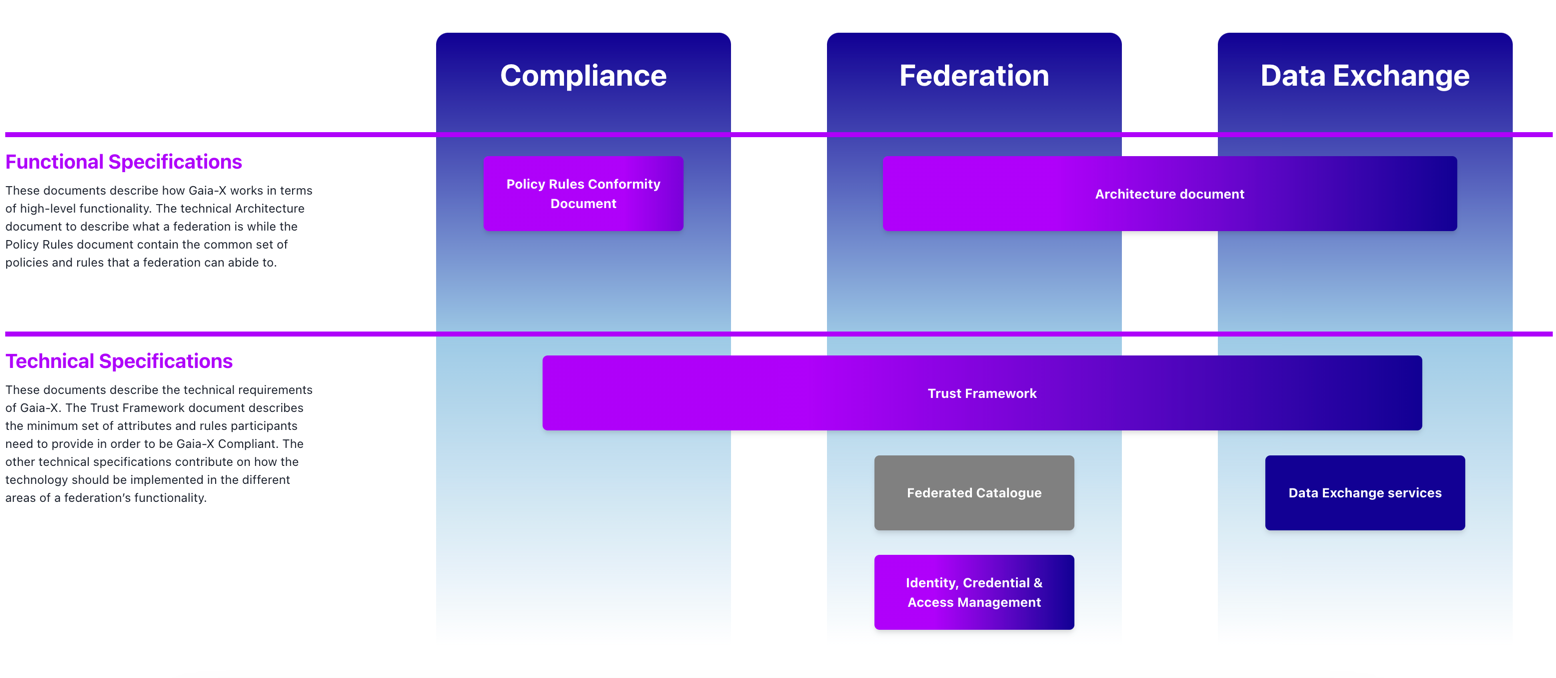
\includegraphics[width=\textwidth]{figures/specifications.png}
    \caption{Gaia-X specifications divided into functional and technical groups and ``Compliance,'' ``Federation,'' and ``Data Exchange'' blocs~\cite{gaiax}.}\label{fig:specifications}
\end{figure}

An issue arises from this division as multiple documents often describe the same components, leading to inconsistencies.
For example, the \textit{DataProductDescription} credential described by the ``Data Exchange Document''~\cite{gaiax_data_exchange_document} is supposed to be inheriting attributes of the \textit{ServiceOffering} credential, defined in the ``Trust Framework,''~\cite{gaiax_trust_framework} but the common attributes do not match.
Following is an example of mismatched attributes in the format (\textit{service offering attributes}) vs. (\textit{data product description attributes}): (\texttt{name}, \texttt{policy}) vs. (\texttt{title}, \texttt{hasPolicy}), respectively.

Another issue with the ``Data Exchange Document''~\cite{gaiax_data_exchange_document} specification is a wording mismatch between the component in the specification (\textit{DataProduct}) and in the XFSC implementation of the DCT (Data Contract Transaction) service (\textit{DataAsset}).

Yet another inconsistency surrounding the specifications concerns the policies.
The ``Data Exchange Document''~\cite{gaiax_data_exchange_document} states that the allowed policy languages are \textit{Rego}, \textit{ORDL}, and \textit{XACML}\footnote{\url{https://groups.oasis-open.org/communities/tc-community-home2?CommunityKey=67afe552-0921-49b7-9a85-018dc7d3ef1d}}, whereas other documents only mention \textit{Rego} and \textit{ORDL}.
Additionally, the \textit{Rego} policies are evaluated against a given input.
Still, in the case of Gaia-X, the attributes that are part of the input object need to be clarified, and I couldn't find the definition in any of the specifications.

The specifications are also often vague about posed requirements.
The attributes of objects are typically defined in tables and can be standalone Gaia-X credentials or just objects that are part of the credentials.
However, this distinction is not always clear.
For example, when the ``Trust Framework''~\cite{gaiax_trust_framework} defines a link to another credential as the attribute, it typically uses a comment like ``a resolvable link to the \texttt{credential} self-description providing the service.''
However, the attribute \texttt{serviceAccessPoint} of \texttt{InstantiatedVirtualResource} is described as ``a list of Service Access Point which can be an endpoint as a mean to access and interact with the resource.''
This description implies a simple embedded object, but in reality, a link to the credential is expected.

I argue that Gaia-X should make efforts to remove the inconsistencies between individual specifications.
Merging the different documents into a single large one could be beneficial to remove redundant definitions, which can cause inconsistencies.
Another approach could be creating an additional overarching document, which would explain the ``bigger picture'' of the Gaia-X ecosystem and explain the necessary components from the point of view of different user roles (Federator, Provider, Consumer).
A ``getting started'' section with Gaia-X, commonly used by many software libraries and frameworks, along with minimal examples of the usage, could bring much value to newly onboarding users and smoothen out the experience.

\subsection{Gaia-X Digital Clearing House}\label{subsec:gaia-x-digital-clearing-house}

The GXDCH is a set of running services consisting of Compliance, Notary, and Registry, which operationalize the rules stated by the Gaia-X specifications.
As with the specifications, they are not free from their own set of issues.

The main issue surrounds the imperfect alignment with specifications.
For example, the Notary service currently only validates a \texttt{LegalParticipant}'s registration number and issues the \texttt{LegalRegistrationNumber} upon providing a valid registration number.
The ``Trust Framework''~\cite{gaiax_trust_framework} document specifies five admissible types of registration numbers --- \texttt{local} (state-issued), \texttt{EUID}, \texttt{EORI}, \texttt{vatId}, and \texttt{leiCode}.
The Registry, which formalizes credential structure, recognizes \texttt{taxID} instead of the \texttt{local} registration number.
However, when presenting a state-issued registration number under either of these options, both lead to the Notary returning an error.

Another misalignment between the specifications and the formal Registry's implementation concerns the \texttt{LegalPerson} Gaia-X credential.
The \texttt{legalAddress.countryCode} attribute doesn't match the formalized version \texttt{legalAddress.countrySubdivisionCode}.

The formalized version of the \texttt{DataResource} credential in the Registry's DB seems to be incorrectly aligned with the ``Trust Framework''~\cite{gaiax_trust_framework} specification definition.
In the document, the \texttt{exposedThrough} attribute expects a resolvable link to the \texttt{InstantiatedVirtualResource} credential, whereas the Registry expects a link to the \texttt{ServiceOffering} credential.
This discrepancy leads to the inability to obtain Compliance for \texttt{DataResource}/\texttt{ServiceOffering}-related Gaia-X credentials.

Another major issue with the Registry and Compliance services is the missing implementation of Gaia-X credentials defined in their respective specifications.
As an example, the ``Trust Framework''~\cite{gaiax_trust_framework} document defines two types of \texttt{Participant} credentials, \texttt{LegalPerson} and \texttt{NaturalPerson}, but the Compliance and Registry services only implement the \texttt{LegalPerson} at the moment.
The ``Architecture Document''~\cite{gaiax_architecture_document} also defines three roles for a participant (Provider, Consumer, Federator), which have not yet been implemented.
This missing implementation is, however, acknowledged in the ``Trust Framework''~\cite{gaiax_trust_framework} document.

Importantly, the data exchange-related credentials are also not implemented in the Registry's trusted DB, which means that none of the credentials defined in the ``Data Exchange Document''~\cite{gaiax_data_exchange_document} can be validated and receive Compliance.
Additionally, the possibility of notarizing the \texttt{DataProductUsageContract} credentials is another use case described by the ``Data Exchange Document,''~\cite{gaiax_data_exchange_document} which is not implemented by the Notary.

One of the less severe but still notable inconsistencies is the naming of the GXDCH services' endpoints.
The Compliance uses \texttt{kebab-case} for endpoint routes, the Notary uses \texttt{camelCase}, and the Registry combines both conventions.

I believe Gaia-X should work intensely to ensure that the implementations, including the credential vocabulary's formalization, conform to the predefined specifications.
Clearly marking the features, which are not yet implemented and exist only as specifications, would help adopters immensely to save time and resources.

I also find the benefit of validating legal entity registration numbers debatable.
This belief is based on the fact that the test only asserts the validity of said registration numbers and not their affiliation to the respective legal person.
This does little to help establish trust among Participants and introduces a dependence on a centralized service (EU-run API is used for validating VAT ID). During my developmental phase, the API for validating VAT ID was often inoperational, leading to Compliance's service's inability to provide Compliance for the Participant-related credentials.

A feasible alternative may be validating a registration number based on the attributes included in the legal person's certificate.
This fits well with Gaia-X's requirement to use qualified certificates regulated by the eIDAS Regulation (EU) No 910/2014, which stipulates that \textit{``Qualified certificates for electronic seals shall contain at least the name of the creator of the seal and, where applicable, registration number as stated in the official records;''}~\cite{eidas}.
This approach would guarantee the participant's affiliation to the provided registration number, increasing trust.

\section{Cross Federation Services Components}\label{sec:cross-federation-services-components}

Cross Federation Services Components (XFSC) is the reference implementation of concepts and workflows defined by Gaia-X specifications.
It includes the services operated by GXDCH.
It includes core services for data exchange (``Data Connector'') and for setting up federations, like the ``Core Catalogue Functions,'' and ``Orchestration.''
Additionally, they provide tools like the ``Self-Description Wizard,'' ``Personal Credential Manager,'' ``Organization Credential Manager,'' and ``Data Exchange Logging Services.''
Different services are in various development phases, as the Gaia-X website~\cite{gaiax} indicates in a visualization.
Some services are still in development, as indicated by their box being greyed out; others, like Compliance, Registry, and Notarization services, are already released.
The development status differs by the selected version, where most services are developed in version \textit{21.03}.

The initial goal was to use the ``Data Connector'' service to exchange data between Carecentive and data consumers.
However, because the ``Data Connector'' service has not yet been released in any of the versions, the focus was changed to providing data using Carecentive's existing API.
To enable data consumption over the existing API, the aim was to utilize the ``Data Contract Services'' to establish the initial handshake between Carecentive and the data consumer.

``Data Contract Services'' implement data exchange and contracting workflows as defined in the ``Data Exchange Document''~\cite{gaiax_data_exchange_document}.
The intent was to use version \textit{21.03}, since it's the only stated release of the service, and integrate it into the running stack of Carecentive.
However, upon examining the service's repository and setting it up, it was discovered that while the service seems functional initially, the API has hardcoded responses to predefined requests.
In conclusion, crucial internal components are missing from the service, which renders the ``Data Contract Services'' unusable.

It is necessary to mention that coming up to this conclusion was hindered by the incorrectly visualized release status.
Furthermore, the visual representation of services links to an old Gitlab group, which was migrated to the Eclipse Foundation Gitlab account, leading to the need to search for the correct repository.
The links should be updated to redirect to the correct respective repositories and ideally to the correct branch or commit marking the release.
The correct linking would significantly simplify the adoption process for developers.
Additionally, the documentation/README files should be improved, as in the case of DCT, the README file consists mainly of an unmodified template.

To mitigate the issue with unfinished implementation of the DCT, a simplified version inspired by the contracting workflow of the ``Data Exchange Document''~\cite{gaiax_data_exchange_document} was implemented directly into the Carecentive platform to enable data exchange functionality.
The exact workflow is detailed in Section~\ref{subsec:data-contracting}.
Unfortunately, this meant that I was unable to test features related to a missing policy engine, like policy enforcement and contract negotiation.

Gaia-X should provide correct information on the development status of XFSC services and update the links to lead to the proper repositories.
Adopting developers would also benefit significantly from improved documentation of the XFSC services.

\section{Experiments}\label{sec:experiments_discussion}

Six experiments were designed to test the implementation of the data exchange module and evaluate the feasibility of the Gaia-X ecosystem for exchanging data, particularly in medical trials.
Three of the six tests were carried out successfully, two failed, and one couldn't be conducted due to the missing XFSC component --- the ``Data Contract Services.''

The two failed experiments both verified the process of obtaining Gaia-X compliance for the data resource and data exchange-related Gaia-X Credentials.
Their failure showcases that the maturity of the Gaia-X project is low, as the concept of Gaia-X Credentials is a central part of the project.
The missing XFSC component, leading to the inability to conduct experiment no.~6, also shows that the project is still very much in active development.

Experiment no.~1 demonstrates that the very core feature of onboarding Participants is functional, but currently, it is only limited to legal entities and not natural persons or other types of Participants.
It is unlikely that in the current developmental lifecycle, the Gaia-X can accommodate non-trivial use cases.

Test cases no.~4 and 5 showcase that while the data exchange is possible, at the moment, additional efforts in developing parts of the missing functionality or utilizing non-Gaia-X protocols are necessary.
These tests are evaluated as passed as they are based on Gaia-X specifications and lead to a successful exchange of data.
However, since they are based on credentials which could not be issued compliance for and therefore were not validated, the process cannot be though of as Gaia-X-compliant.
The absence of Gaia-X-compliance is underlined by the fact that the key features advertised by the ``Data Contract Services,'' such as policy enforcement and contract negotiation, are not implemented in the simplified version of the contracting service.

To answer research question 1 --- ``\textit{Is it feasible to share healthcare data in Gaia-X Data Spaces?}'' --- the answer is currently no.
The reasons are the missing XSFC components and inconsistencies between specifications and running GXDCH services.
